\chapter{Data requirements for statewide modeling}

Statewide models require many of the same data as those deployed in urban and metropolitan areas, owing in part to the similarities of the underlying models. However, the scale is different, as is the representation of external markets. Many statewide models now include a national coverage of zones, at lower levels of resolution as the distance from the state increases, as well as explicit representation of visitor travelers. These increase the data burden for statewide model developers and users. Fortunately, considerably more data are available for such broader coverage, reducing the cost of building and maintaining statewide models. 

The many types and levels of data required in statewide modeling are discussed in this chapter. The macroeconomic and geographic contexts are discussed in the next two sections, followed by a discussion of the transportation networks represented in such models. This is followed by a discussion of how data on personal travel behavior and choices are collected, from both traditional and newly emerging sources. A similar discussion of traditional and non-traditional freight data sources and opportunities follows it.

\section{Macroeconomic linkages}

Explicit linkages to macroeconomic models are becoming an increasingly important part of state\-wide models. While still rare in metropolitan travel forecasting models, they have a long history in statewide modeling. Michigan was one of the first states to incorporate the REMI model into their process, over 35 years ago. Several other states have used them for an equally long time. \cite{sorratini00} describe how they used both economic forecasts and input-output (IO) coefficients to improve their commodity flow model in Wisconsin. Such models are typically developed independently, and are used in conjunction, rather than tightly integrated, with the travel forecasting models.

Economic models typically fall into one of two categories. The more traditional category includes macroeconomic forecasts that are typically inputted to the statewide model. However, economic impact models are increasingly being used as well, as described in \S\ref{sec:economic-impact-models}. They can be used singly or in combination. Most operate separately from the statewide model, but are included in the statewide modeling system in a few instances.

%\protect\hypertarget{h.av9jpbxyqir7}{}{}

Economic forecasts for broad areas and industry categories are used to generate estimates of future socioeconomic activities within the modeled area. These appear to be done most often at the statewide or sub-state region level, with modelers allocating them further to counties or traffic analysis zones based upon existing zonal employment estimates, land use data, accessibilities, and other measures.

Firms and employment are most often coded to the two-digit NAICS codes \citep{censusbureau16}. Some states use greater detail for dominate industries within the state, and combine those found less frequently. Others aggregate the two-digit NAICS into families of firm type (e.g., service, retail, manufacturing). Those choices of spatial and industry resolution appear to largely hinge upon data availability.

We found that most states (29 out of 46) reported that they used exogenous economic forecasts in their work, or in the case of eight states no forecast at all. The source of these forecasts varies widely, as does the amount of work going into them. Many reported using forecasts created by the state economist or other state agencies charged with developing them. About a 46 percent rely upon third-party forecasts that are customized, at least in part, to the definition of regions and industry sectors used in the statewide model. There may be cases where these third-party forecasts are also used by other state agencies or instead of official state forecasts, although we did not attempt to quantify such cases.

%\protect\hypertarget{h.jsvny4stsszd}{}{}

\section{Spatial coverages}

Statewide models typically employ a wider range of spatial representations than urban models, in part because of the larger area involved. Various types of data used in model development and application are available only at certain levels of geography, which also dictates the level(s) of resolution used in statewide models. Finally, most statewide models now extend well beyond the state borders, usually with decreasing level of detail as the distance from the state increases. It is common to represent the area within the state and a halo around it with traffic analysis zones that aggregate to counties and Census geographies. Outside of the state successively coarser political and Census geographies are used to represent distant markets. FAF regions, described in \S\ref{sec:traditional-freight-data}, are being increasingly used to represent external markets. Many of the models reviewed use multiple levels of geography during implementation, and for communicating results.

Arguably nowhere is the tension between the number of zones and computational burden felt more acutely than in statewide modeling. In smaller states, it might be possible to ``stretch'' the urban models to cover the remainder of the modeled area, with no loss of resolution or precision in the former. However, this is not practical in most cases, for the run time of most models increases geometrically as the number of zones increase. Even on the best hardware available today advanced models with 7,500 or more zones are cumbersome and slow, with formidable resources required for developing and maintaining data that level of geography. Thus, most statewide models aggregate the zone systems used in urban models where they overlap, and add zones in the areas not covered by them.

A definitive best practice for integrating urban and statewide zones remains elusive. In some cases, groups of urban zones are nested within each statewide zone. Equivalency tables are used to transfer information from one zone system to the other if needed. In other cases, processes for defining unique statewide zones are used. The process for conflating different polygon coverages using GIS software is relatively straightforward. This reduces, if not eliminates, the need to keep the boundaries of urban and statewide zones synchronized.

Automated processes for generating zones can be used for those willing to relax the requirement for exactly matching urban zones (or groups thereof). \cite{moeckel15a} described a process for automatically generating grid cells of varying size, depending upon the underlying levels of household and employment density. This was used to create an alternative zone system for the Georgia statewide model that significantly improved the assignment results, based solely upon the new zone system. 

A variant of this gradual rasterization process has been employed in Ontario, where instead of successively dividing a single cell covering the entire state the process starts with grid cells 50 miles (80 kilometers) on each side covering the province. Each cell is successively divided into four smaller cells, until a threshold activity density or minimum zone size is obtained. This precludes huge zones in Ontario's sparsely populated northern areas. Another variant has been implemented for the Munich metropolitan area, where jurisdictional boundaries were respected. Here, gradual raster cells were created and intersected with municipal boundaries. Resulting small slivers of raster cells that were cut by municipal boundaries were merged with other raster cells within the same municipal area to avoid small pieces of raster cells.

The use of microsimulated synthetic households has become standard practice in activity-based travel modeling. They can be used with traditional trip-based models as well, opening new possibilities for either simulating travel between point locations, or for developing new methods for organizing them into polygons (zones) based on homogeneity of household characteristics (e.g., accessibility to certain travel modes, uniform density patterns). The prospect of simulating travel from point locations instead of zones is not as preposterous as it might seem. National models of Germany and Switzerland were implemented in MATSim using this approach \citep{balmer08}.

Modeling travel between point locations will not obviate the need for zones. It will, however, relax the requirement for the latter to be as deliberately designed for compatibility and uniform activity size or land area as traditional models. The provincial model currently under development in Ontario is based on synthetic households and firms, yet still uses at least two different traffic analysis zone systems. The latter are used to represent skim matrices, accessibilities, and centroid connections to macroscopic traffic assignment models. Certain spatial patterns, such as density, accessibility, parking costs and area types are more efficiently displayed and comprehended in aggregate than individually. The tracing of individual flows in microsimulation-based travel models is useful for modelers. However, it seems unlikely the advantages associated with aggregating data for visualization will diminish, at least when communicating modeling outcomes to non-modelers. Thus, ``the tyranny of zones'' \citep{spiekermann99} appears to be with us for the foreseeable future.

\section{Network representations}\label{sec:network-representations}

Abstract representations of the multimodal transportation system are included in statewide models. These include the networks used by each mode of transport represented in the model, for both personal and commercial travel. It also includes intermodal connectors, border crossings, major freight generators, and in most cases, an external network that connects the states to major external markets. These external networks often become highly aggregated, often to only Interstate and federal highways and major rail corridors as the distance from the state increases.

Most states build their internal roadway networks from geodatabases maintained by GIS teams within the agency. Most originated from centerline coverages and roadway geometric data. These are most often linked to Highway Performance Management System (HPMS), traffic monitoring, and other performance monitoring databases used in the agency. The initial development of the network is often an ad hoc exercise, for once built it is typically used for a long time. Such networks are often refined, either in their source data or just in the statewide model, but the lack of funding for large infrastructure projects has reduced the amount of work required to build and maintain a time series of planned network improvements.

Building a roadway network from existing data source seems conceptually simple, yet it was widely reported as the most time-consuming and frustrating part of building the model. Several reasons were cited:

\begin{itemize}
\item
GIS line layer representations do not easily translate to the directional links used in most travel models. Most third-party modeling platforms include utilities for converting line layers to transport networks, but they rely upon an exact and consistent manner of GIS layer coding that is rarely found in practice. The endpoints of many links do not exactly coincide with those of upstream and downstream links, and often allow movements that cannot be made in reality.
\item
Traffic models require link attributes that are not included in DOT roadway inventories, such as capacity, free flow speeds, and permissible lane use (e.g., parking or turn-only lanes).
\item
GIS networks are not navigable, and thus, their connectivity and proper coding of directionality, the number of lanes, and other attributes have never been rigorously checked.
\item
State DOT databases often lack important streets within urban areas, or have different attributes than those coded for the same roadways in urban model networks.
\item
Traffic count data are stored in different systems than geometric data, and require considerable work to combine with the model networks.
\end{itemize}

Correcting these problems, and addressing related issues, was identified as the single largest cause of delay and cost overruns when building statewide models. Maintaining these networks was also cited as a major resource requirement that distracted from efficiently responding to requests for forecasts and analyses.

The amount of work involved in building internal roadway networks has led some states to explore the use of automated conversion of Open Street Map (OSM) data. This process still requires some manual intervention, as some attributes needed in network assignment are missing, and there is no guarantee of network connectivity. Moreover, rural networks are often not as quickly updated as urban ones, which enjoy a larger group of committed users. Thus, while OSM solutions have been applied in research settings (compare \cite{ziemke16} for the state of Maryland), no state appears close to having successfully used it as the officially sanctioned source of internal network data.

Ironically, building the external highway network, as well as networks for other modes of transport, is often much easier. Many states use the National Highway Planning Network developed by USDOT or the Oak Ridge Network, developed for coding and analysis of national freight data sources, for this task. They are already coded in the format required for travel forecasting, although lack the level of detail required within the target state. The National Rail Network is likewise often used, sometimes in conjunction with more detailed network data from Railinc. Pipelines are often omitted, and marine and air networks and ports are small enough that they are easy to code using federal data sources.

A gray area in the middle is the representation of public transit. Fixed guideway transit systems are relatively easy to code, for both urban and intercity systems. Except for the Northeast and West Coast, the intercity public transportation networks are relatively sparse. Federal sources of network data are lacking, but these can typically be coded from metropolitan and carrier-provided network data. General Transit Feed Specification (GTFS) data are now routinely used by some agencies to automate the coding of fixed guideway transit networks and their service characteristics.

A thornier aspect involves how local bus transit services are included in statewide models. While they can now be coded much faster and more accurately using GTFS, their addition to statewide models remains problematic. The larger zones and coarser urban travel market segments make the coding of access and egress more difficult and less accurate, and the need to include local streets that buses run on can greatly increase the number of links required in the model. This, in turn, imposes an additional computational burden, especially for path-building in highway and transit assignment. Thus, even if GTFS could automate what would otherwise be a hugely onerous network coding task, would the results be worth the effort? Two different approaches have emerged that offer a tractable alternative:

\begin{itemize}
\item
\cite{circella13} developed a process for building an abstract representation of likely local bus accessibility, based upon urban form characteristics. The approach was initially developed in Oregon, and later improved during its implementation in California. Zone-to-zone bus travel times are calculated as a function of auto interzonal travel times. Assumptions about fares and service levels must still be made by the user, but robust bus travel times can be estimated using the coarser networks typically found in statewide models.
\item
Logit averaging can be used to represent composite impedances and accessibilities from urban models, where bus transit is modeled explicitly, to statewide models. This obviates the need for network coding, as the mode choice logsums are computed on a zone-to-zone basis, but are not influenced by how the zones are designed. This approach is being used in HSR forecasting in Texas.
\end{itemize}

Both approaches offer tractable and affordable alternatives to maintaining extensive local transit networks, which typically only play a small role in intercity and major statewide flows.

\section{Traditional personal travel behavior data}\label{sec:traditional-person}

Statewide models typically include a wider range of diverse travel markets than traditional urban models do, increasing their data requirements for model development and application. Visitor travel, for example, is often explicitly represented within statewide models at varying levels of fidelity and resolution. Moreover, statewide models must accommodate the diversity of travel behavior and choices by residents living in metropolitan, suburban, small towns, and rural areas. Merely enumerating these markets can be challenging in some cases, much less the collection of data about them, and accommodating such within a single modeling framework.

The behavioral data used in statewide models came primarily from four sources, as shown in Figure \ref{fig:behavioral-data-sources}. The NHTS was used by almost two-thirds of the states that reported what type of behavioral data they used in building and applying models. Household travel surveys were used by almost half of the states, while synthetic and transferable rates compiled in various NCHRP reports were used almost as frequently. Passively collected data, described in the next section, was reportedly used by a quarter of the states.

\begin{figure}   % 40
\centering
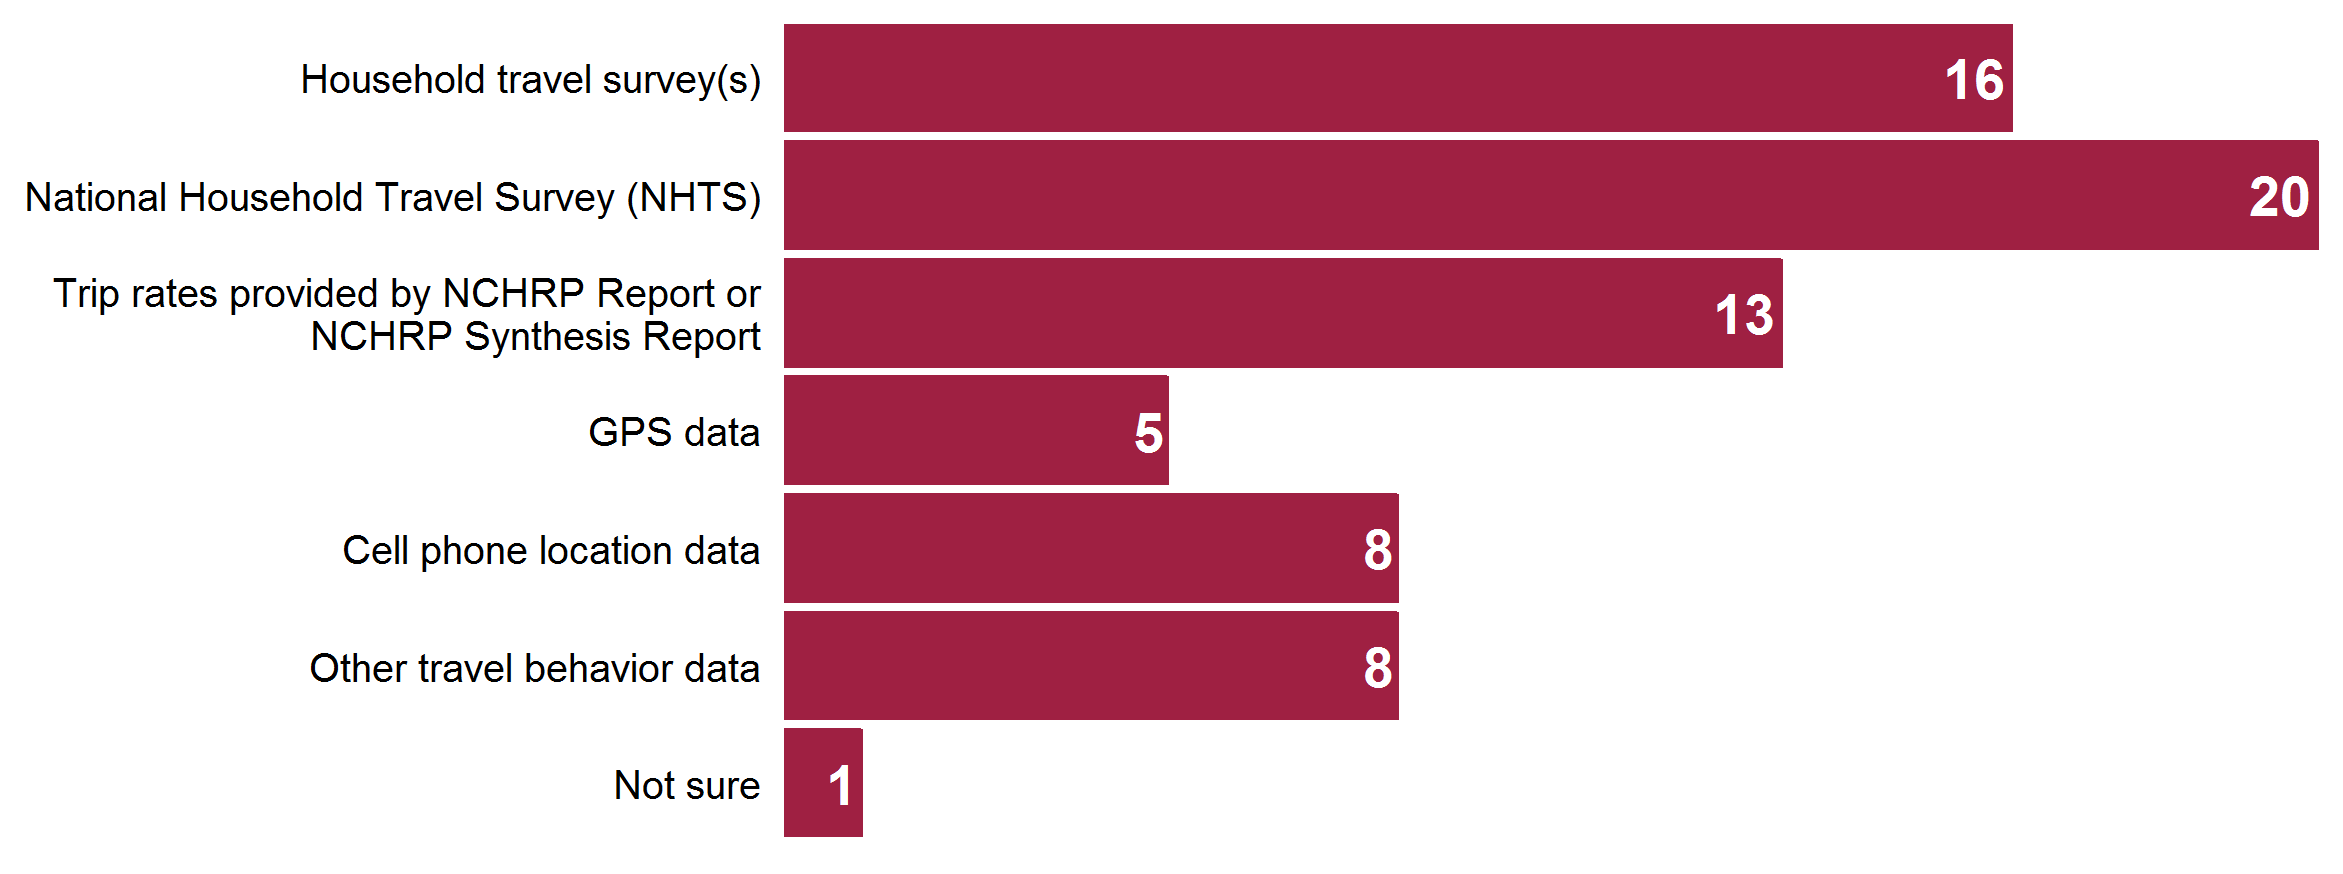
\includegraphics[width=6.4in]{graphics/40-behavioral-data-sources}
\caption{Behavioral data sources used for building statewide models}
\label{fig:behavioral-data-sources}
\end{figure}

Most states reported using multiple data sources. However, the ways these data were combined reveal almost no pattern of standard practice, as shown in Table \ref{tab:data-combinations}. The exclusive use of the NHTS by a quarter of the states is surprising, and indicates its importance in statewide modeling. Five states reported using only household travel surveys for model development, which is also surprising, given the additional markets covered in most statewide models that such surveys do not illuminate (e.g., visitors, long-distance travel). However, four of them --- California, Michigan, Ohio, and Oregon --- conducted statewide surveys that provided data for all households across the state, reducing or obviating their need to supplement their survey data. The characteristics of the surveys conducted by these four states are summarized in Table \ref{tab:comprehensive-surveys}.

\begin{table}   % 3
\centering
\caption{Combinations of data used to build statewide models}
\label{tab:data-combinations}
\begin{tabular}{lrr}
\hline
Data source(s) used & n (states) & Percent \\
\hline
National Household Travel Survey (NHTS) & 7 & 24.1 \\
\gray Household travel survey (HTS) & 5 & 17.2 \\
HTS and NCHRP rates & 2 & 6.9 \\
\gray HTS and passive data & 2 & 6.9 \\
HTS and NHTS & 2 & 6.9 \\
\gray HTS, NHTS, and NCHRP rates & 2 & 6.9 \\
NHTS and NCHRP rates & 2 & 6.9 \\
\gray NHTS and passive data & 2 & 6.9 \\
NHTS, NCHRP rates, and passive data & 2 & 6.9 \\
\gray NCHRP rates and passive data & 2 & 6.9 \\
NCHRP rates & 1 & 3.4 \\
\hline
Total & 29 & 99.9 \\
\hline
\end{tabular}
\end{table}

\begin{table}
\centering
\caption{Comprehensive statewide travel surveys}
\label{tab:comprehensive-surveys}
\begin{threeparttable}
\begin{tabular}{llclrr}
\hline
State & Survey & Year(s) & Survey Type\tnote{a} & Households & Cost\tnote{b} \\
\hline
Ohio & Household Travel Survey & 2003 & 24-hour HTS & 15,000 & \$2.0M \\
\gray Ohio & Long Distance Travel Survey & 2003 & 2 week RTS & 8,000 & \$0.4M \\
Michigan & MI Travel Counts I & 2004-05 & 48-hour HTS & 14,966 & \$2.1M \\
\gray Michigan & MI Travel Counts II & 2009 & 24-hour HTS & 1,975 & \$0.52M\tnote{c} \\
Oregon & Oregon Travel and Activity Survey & 2009-11 & 24-hour HTS & 18,282 & \$3.6M \\
\gray California & California Household Travel Survey & 2012-13 & 48-hour HTS & 42,431 & \$10M\tnote{d} \\
California & California Household Travel Survey & 2012-13 & 2 month RTS & 18,012 &  \\
\gray Michigan & MI Travel Counts III & 2015 & 24-hour HTS & 16,276 & \$2.4M \\
\hline
\end{tabular}
\begin{tablenotes}
\footnotesize
\item[a] HTS = household travel survey, RTS = retrospective (long-distance) travel survey
\item[b] Current dollars in the year the survey was contracted
\item[c] Higher cost attributable to inclusion of an attitudes and perceptions add-on survey
\item[d] Cost shown includes both household and retrospective survey
\end{tablenotes}
\end{threeparttable}
\end{table}

The four statewide surveys are notable in their scope, covering the entire state. They also featured large sample sizes and use of common sampling approach and instruments across the state. Most were stratified to obtain usable sample sizes for different areas of the state or area type (e.g., metropolitan, small urban, rural) in addition to the usual stratification by household attributes. The findings typically reveal different travel patterns by sub-state areas. In Oregon, for example, rural residents make fewer but longer trips, with more intermediate stops than urban residents. Applying urban patterns to the remainder of the state would result in significant errors or incorrect policy sensitivities. Thus, these large-scale surveys are a sound investment. Moreover, collaboration with the MPOs within each state results in a common approach to conducting such surveys, enabling each to obtain a large sample of usable observations than either could afford alone.

Not shown in Table \ref{tab:comprehensive-surveys} is a new statewide survey getting underway in Ohio as this report was being finalized. They are planning to spend approximately \$7.5 million over the next decade to collect data from 2,500 households per year. Their target is to obtain seven days of data collection for each household, with 70 percent including GPS collection on smart phones. Most notable about their effort is highly rigorous ``zero defect'' requirements for survey completion. Their goal is to eliminate incomplete responses and missing data from certain household members, which if successful will advance the state of practice for all household travel surveys, not just at the statewide level.

Several other states used metropolitan travel surveys, often in combination with other data sources, to build statewide models. In Maryland, for example, urban household travel surveys conducted in different years by the Baltimore Metropolitan Council and the Metropolitan Washington Council of Governments were fused to develop the statewide model. The former had enough samples from suburban counties to help differentiate their differences in travel behavior. However, the biggest differences were in the travel patterns of residents of the two major cities, underscoring the importance of accounting for the unique characteristics of different urban areas within statewide models.

As useful as the statewide travel surveys are, they typically only gather information about daily travel patterns on the survey day(s). They are less useful for understanding certain aspects of travel behavior important in statewide models:
\begin{itemize}
\item Their sample sizes are too small to reveal robust origin-destination patterns
\item Long-distance trips are under-represented
\item Visitor trips are not captured
\end{itemize}

It is widely accepted that household travel surveys are large enough to illuminate differences in trip and tour formation and structure \citep{stopher07}, but too small to reveal origin-destination patterns unique to the surveyed area. Census journey-to-work data at the county level have long been used to better understand commuting flows in statewide models, but are limited to information about that trip purpose, with frequent suppression of smaller interchanges that collectively prove important in understanding flows between urban areas. This is an area, however, where big data are being used to fill that long-standing gap in knowledge. Such opportunities are described in the next section.

Long-distance travel, which takes place less frequently, is rarely captured in household travel surveys in large enough numbers to be useful. Only Ohio and California have administered separate long-distance travel surveys. It is widely acknowledged that two to three-month retrospective surveys are more useful for collecting information about these types of infrequent trips. Unfortunately, there are little national data to borrow from to construct such models. While used extensively in Europe, the last large-scale long-distance travel survey in the USA, the American Traveler Survey, was conducted in 1995. The small long-distance add-ons to the National Household Travel Survey (NHTS), conducted in 2001-02 and 2009, are considered too small to be very useful. This has not stopped modelers from attempting to use them despite their small size, although results have been uneven at best.

The largest time series of long-distance travel data in North America are the Travel Survey of Residents of Canada (TSRC) and International Travel Survey (ITS), both conducted by Statistics Canada. Since its last overhaul in 2010, the TSRC has continuously collected data on long-distance travel, which are available to researchers as microdata. The data are being used to develop provincial travel models in Ontario and Alberta, using different methods in each. They are being used to develop microsimulations of resident and visitor long-distance travel by season in Ontario, whereas model design is just getting underway in Alberta.

The national scope of the TSRC and ITS enable them to be used to build models of both resident and visitor flows. While a work in progress at this writing, preliminary results show important differences in the characteristics and travel patterns in residents of versus visitors to Ontario. The transferability of these models to the USA is an open question. However, the Canadian program provides an encouraging example of a well-run survey that is almost singular in its scope and breadth, as well as utility for building robust statewide models.

The published syntheses of travel data from several NCHRP reports were widely used in building statewide models. These include:
\begin{itemize}
\item NCHRP Report 716, ``Travel demand forecasting: parameters and techniques'' \citep{cambridge12}
\item NCHRP Report 735, ``Long-distance and rural travel transferable parameters for statewide travel forecasting models'' \citep{schiffer12}
\item NCHRP Report 765, ``Analytical travel forecasting approaches for project-level planning and design'' \citep{cdmsmith14}
\end{itemize}

The way in which these reports were used was interesting. Follow-up conversations with respondents who indicated they exclusively used the NCHRP reports did so because funding limitations precluded primary data collection. The states that used the reports in combination with other data sources, by contrast, primarily used them to glean information about the unique travel patterns of rural residents, develop model calibration and validation targets, and assess the reasonability of delivered models.

Some states employed roadside interviews of motorists in the past, attempting to overcome the paucity of data on long-distance travel. They also used such data to focus on key corridors across the state. Our findings suggest that this practice has largely been abandoned. Interviews had to be completed quickly if done on site, limiting the amount of information collected. Mail-back surveys enabled more data to be collected, but suffered from low response rates. Even where the data were collected on-site the surveys suffered from small sample sizes, inability to control for non-respondent bias, high cost per completed interview, and questionable transferability, even of aggregate summary statistics. However, it appears that legislative or executive prohibitions on the practice, prompted by citizen complaints, effectively ended roadside interviews in most states rather than methodological or data quality considerations.

\section{Non-traditional personal travel behavior data}\label{sec:nontraditional-person}

The growth of big data solutions for transport planning applications has arguably had no greater early successes than in statewide modeling. These data are passively and continually collected from cellular and GPS devices, and summarized in origin-destination and travel time matrices and summaries by third parties. Almost a quarter of the respondents who revealed their sources of data reported using AirSage data for model development. These data can fill the gaps in knowledge noted earlier about infrequent long-distance travel, as well as revealing origin-destination patterns within the modeled area. It is important to note that the AirSage data do not represent the universe of big data solutions, and arguably might not be the biggest player in that rapidly expanding market. However, they were the most frequently cited vendor. The experiences reported provide useful insights that will likely apply to many big data products used in statewide modeling.

Some details of how AirSage collects and processes data are proprietary. What is known, however, is that they receive a time-stamped position record every time a transaction with a Verizon or Sprint device occurs. Some users rarely use their mobile phones, but most have a variety of applications always active, ensuring a constant stream of location coordinates from a customer base that is estimated at half the cellular phone market in the USA. Given that mobile phones are almost ubiquitous this equates to a continual stream of travel tracking data from about half of the population, over several years. Simple heuristics can be applied to the raw data to identify the likely home and work or school locations, based on when, how often, and how long they repetitively visit certain locations.

It does not appear that AirSage attempts to fuse their data with business location, household, or land use information to further infer what activity the traveler is engaged in during each stop. Nor is it clear how they identify (activity) stop locations in the first place. However, with few exceptions their ability to differentiate home-based work, home-based other, and non-home-based trips should be robust, especially at the level of spatial resolution in most statewide models. Some users have questioned the validity of the data at fine levels of geographic resolution, or ability to use it for constructing tour-based models (where identification of intermediate stops is important). However, these are likely to be outside of the interests of most statewide modelers. Moreover, the broader levels of spatial resolution and trip purposes do not distract from the value of the data for model validation or reasonability checking.

Because the typical home location of the otherwise anonymous user is known it is easy to know when they travel outside of their normal area, or to pinpoint long-distance commuters. This enables AirSage to create a visitor trip matrix for any given study area, to include information such as where visitors spend the night, clusters of activity locations during the day, and visit duration (time away from normal area). The value of such data for modeling visitors in statewide models cannot be understated.

Several other vendors have entered the big data market, including INRIX and StreetLight. They use alternative sources of information or add data and value to the raw AirSage data. Both can provide data on internal travel times, or at least for larger origin-destination flows, which AirSage does not. Even though these big data sources lack characteristics of the traveler (other than what can be inferred from where they live and work) and the trip, they remain invaluable for statewide modeling. Reliable and robust OD patterns for both residents and visitors can be constructed from these data, whose sample size is at least two orders of magnitude larger than any known household travel survey. The latter cannot provide reliable OD patterns except at very coarse geographic levels, while the former can easily work at the level of the coarse zones typically used in statewide models.

It must be acknowledged that cellular tracking data are less than ideal on their own. They include no information about the trip or trip-maker, with whom they travel and why, or mode of transport. The latter can be inferred when only a single mode is available or practical, or when certain speeds are reached. However, such analyses would require access to the raw data and considerable additional analyses, which are not available to modelers. Thus, they have become indispensable for statewide modeling, but only when fused with the traditional data described in the previous section. Several innovative uses of these data were reported at the TRB Innovations in Travel Modeling 2016 conference, but have not made their way into the literature at this writing.

\section{Traditional freight travel data}\label{sec:traditional-freight-data}

Understanding long-distance freight movements is often as important in statewide modeling as depicting personal travel. Interstate trucking is often a high percentage of flows on Interstate highways, and exerts a disproportionately high impact on them. There is a long history of modeling inter-regional commodity flows within the USA, some of it quite sophisticated even by today's standards. However, data on freight flows, especially for trucking, have historically been elusive, especially at the level of geography used in statewide models. Most of the data are from federal sources, and are aggregated to large sub-state or statewide regions before release.

While the Commodity Flow Survey (CFS) provided a long time-series of information about domestic flows from shippers in certain industry categories, the data were only available in summary tables until 2015. Many flows were masked due to confidentiality requirements or concerns about sampling errors, making the construction of OD matrices by mode of transport and commodity group difficult, if it could be done at all. The flows were measured in annual dollars (of commodity value) and tons, rather than the weekly or daily vehicle flows by mode needed by modelers.

A variety of approaches were tried over the years to translate annual commodity flows into estimates of traffic by mode, with varying degrees of success. Most gravitated towards a fusion of employment, economic input-output, CFS, and truck count data first proposed by \citep{polenske74, polenske75}. Variants on her approach, as well as means of allocating the flows from counties to statewide model zones, were implemented in several states in the 1980s and 1990s, mostly in the Upper Midwest. Michigan and Wisconsin have tried several approaches over the past forty years. They all required custom code and a wealth of borrowed data fused in an ad hoc manner.

All of that changed with the introduction of the Freight Analysis Framework (FAF), originally developed by FHWA in 1997-99 as a tool for federal policy analyses. It has undergone three significant revisions since, with the first release of Version 4 in 2014. The initial version was a proof of concept, which has undergone significant enhancements in the intervening years. The CFS is the backbone of the FAF, and each major update has coincided with the release of the latest version of the CFS. However, considerable value is added to the data by fusing them with other data, to include the Carload Waybill Sample rail data, domestic and international waterborne commerce data, air freight data compiled by the USDOT, foreign trade statistics, and the Vehicle Inventory and Use Survey (discontinued by the Census Bureau after release of the 2002 survey data).

Unlike the CFS, recent versions of the FAF provide a comprehensive database of freight flows rather than limited static tabulations. Two principal databases are produced:
\begin{itemize}
\item
Origin-destination flows of freight by commodity and mode of transport, measured in tons, value, and ton-miles. These are provided at the county level or international gateway for users within the USDOT, and at the level of FAF regions or international gateway markets for all other users.
\item
Estimates of flows on major routes and segments of highways, by mode of transportation. A range of tonnage is provided at the route level, while truckload equivalents and tons of truck-carried freight are available for segments. Additional attributes are available to USDOT users, such as the commodity and origin-destination data.
\end{itemize}

The FAF is not so much an analytical framework --- a phrase that suggests underlying models --- as it is a commodity flow database. There are no user-accessible analytical methods or products embedded within the FAF. No mode choice model is included, nor are any other policy-sensitive models. Consequently, existing patterns and trends are extrapolated into the future. This can hardly be construed in a negative light, considering that existing choices and preferences remain invariant in most travel demand forecasts. Moreover, the amount of progress made over the past several years is remarkable nonetheless. Perhaps most importantly, the FAF can be used with statewide or national freight models in a far easier manner than the CFS alone.

FAF Version 4 data are available for its base year of 2012, and forecasts in five-year intervals from 2015 through 2045. The forecasts are based upon an exogenous forecast by region in the USA compiled by IHS Global Insight and assumptions about changes in markets and technologies over the forecast period. The economic forecast in Version 4 was widely welcomed, as it was the first FAF forecast to incorporate the effect of the 2008-09 economic downturn and subsequent recession. All modes of freight transport are included in the FAF. Like the CFS, commodities are classified using the Standard Classification of Transported Goods (SCTG) system \citep{bts15}.

The FAF is not without its limitations. Several modelers cited its questionable accuracy, especially when the inter-regional flows are translated into truckload equivalents. Some states report that the data appear quite reasonable, and match heavy truck counts on their borders within acceptable margins. Others report much wider errors. Another lingering and often cited limitation of the FAF is its coarse level of spatial resolution. The data are available at the county level for internal use within the USDOT. However, they are substantially more aggregated when released to all other users, who can only obtain information at a much coarser geographic scale. The 132 FAF regions within the USA nest within states, and counties nest within FAF regions. While the data are still more aggregate in nature than many state and local planners need, it represents a significant improvement over the CFS. Several major metropolitan areas are included in the regions, allowing flows affecting these areas to be more accurately represented.

The FAF is an excellent and important data source for statewide models despite these limitations. Its availability has fundamentally changed the way most states approach freight modeling. Some still rely upon bespoke models or third-party data, but most use the FAF today. Its transparency, greater level of detail, availability of forecasts, and online documentation make it easy to incorporate into statewide models. Several techniques have been developed to disaggregate flows between FAF regions to flows between counties, or even between statewide model zones. The methodologies have traditionally been developed on a case-by-case basis, and are rarely published. Most approaches use one of two procedures, singly or in combination:

\begin{itemize}
\item
Multiple Regression: Commodity-specific flows into and out of a FAF region are used as the dependent variable and employment by type are used as the independent variable. Linear multiple regressions are used to estimate parameters that help explain which employment types generate and attract flows of a given commodity. These parameters are used to disaggregate to smaller zones within a FAF region.
\item
Input-Output Coefficients: Such coefficients describe which commodities are consumed and produced by a given industry. Multiplying employment by type with the corresponding IO coefficients generates a weight for every region that can be used to disaggregate FAF flows.
\end{itemize}

Both methodologies have been applied widely and appear to generate comparable results, at least at the level of the assignment. The former approach has the limitation that parameters are estimated based on large FAF regions with a homogeneous industry mix across the country. The latter approach relies on input-output coefficients that commonly are estimated as dollar flows, while freight flows usually are processed as weight-based flows.

Like the CFS, the FAF expresses freight flows in annual value and tonnage terms. \cite{battelle12} developed a framework for estimating truckload equivalents of the OD flows by tonnage, to include imputation of empty vehicle backhauls, which appears to be used to generate weekly or daily truck flow estimates.

The proprietary Transearch database of commodity flows is similar in structure and coverage to the FAF. It was originally developed by Reebie Associates, but was acquired by IHS Global Insight in 2005. They have continued to offer the same product, as well as bundle it with other consulting services and data subscriptions. Earlier versions of the Transearch database were thought to be based upon the CFS, and supplemented with staff interpretation, addition of additional data from private and third-party data, and surveys conducted by Reebie Associates. Then, as now, the methods used to develop and test the Transearch data are not divulged, nor is information about what the forecast series are tied to. It seems likely that they are tied to IHS Global Insight forecasts, given their present ownership.

The Transearch data have traditionally been offered at a finer level of geographical detail than either the CFS or FAF. The definition of geographical coverages is flexible, and appears to be specified by each client. Within the area of interest, the data are typically provided at the county level and aggregated to approximately 400 Bureau of Economic Analysis (BEA) economic areas, states, or multi-state Census regions outside of it. The ability to customize the level of geographic resolution is an important value added to the Transearch data, even if IHS uses the same methods described above for synthetically allocating FAF data to counties.

Commodities are classified using the Standard Transportation Commodity Codes (STCC), which was used in the CFS before 1997 and is still used by the railroads and in the Carload Waybill Sample. The advantages of the Transearch data include its flexible level of geographic representation, vendor support of the product, and its claimed addition of other data sources to improve the estimates. However, its cost and lack of transparency reduce its utility in model development. Ideally, both data sources could be used to develop statewide freight models, for understanding the differences between the two data products may in some cases be more revealing than singular estimates from either.

\section{Non-traditional freight travel data}\label{sec:nontraditional-freight}

Big data are fundamentally changing our understanding of freight flows, in much the same way they are revolutionizing the analysis and modeling of personal travel. Data about trucking flows and patterns have traditionally been the most difficult and costly to obtain, despite its dominance in freight transport and impact upon roadway infrastructure, road safety, and emissions. 

The introduction of GPS truck tracking data from the American Trucking Research Institute (ATRI) in 2012 has significantly helped to fill that knowledge gap. Like the AirSage data, continuously collected time-stamped coordinates for uniquely identified but anonymous trucks are available. The truck type is unknown, as is the cargo it carries. However, its complete itinerary can be viewed over any desired period. Considerable post-processing is still required to translate the GPS coordinates, and the distance and travel time between them, into stops by duration. Personal travel is typically habitual, limited in the area covered, and occurring within certain hours of the day. Truck travel looks almost random by comparison in many cases, complicating the delineation of tours and stops \citep{sharman11}.

Despite the challenges involved in teasing out discrete tours and stops the ATRI data have been used extensively in statewide models. The use of the data in OD matrix estimation of statewide truck flows has been widely reported in the literature over the past two years. Most use the ATRI data to construct the seed matrix required for the process, requiring the analyst to reduce the data to tours and stops. Many researchers have adopted a rule to define stops based upon the time remains stationary at a given point. Five minutes has frequently been used as a threshold to define a deliberate stop (i.e., to pick up or deliver goods and services, driver breaks, or vehicle maintenance), which seems reasonable for analysis of intercity truck tours. It seems unlikely that a significant amount of cargo could be loaded or delivered in less time.

\cite{bernardin14} describe how they employed this process in Tennessee, with many similar reports appearing in recent literature and conferences. One of the more comprehensive reports, with a detailed description of the tour and stop synthesis process, is a similar report on applications in Florida by \cite{pinjari14}. At least six similar applications have been reported in the literature and at recent conferences. All point to the utility of using these data to describe truck movements across the state, as well as connections to the markets it serves. The fusion of FAF and ATRI data has yet to be reported, but is known to be under development by several researchers.

Other vendors are beginning to offer products for commercial vehicles as well. StreetLight offers data commercial vehicle flows, generated using INRIX data and possibly other sources. Several fleet management systems offer GPS tracking, but have not yet marketed their data for transportation planning purposes. However, the capability to collect and process these data are becoming more ubiquitous, which will likely facilitate more vendors offering comparable products.